\pdfoutput=1

\documentclass[final,leqno,onefignum,onetabnum]{siamltexmm}


\usepackage {algorithm, algpseudocode}
\usepackage {algpseudocode}
\usepackage {amsmath}
\usepackage {amstext}
\usepackage {amssymb}
\usepackage {amsfonts}
\usepackage {mathtools}
\usepackage {makecell}
\usepackage {graphicx}
 \usepackage {tikz,pgfplots}
 \usepackage{subcaption}


\DeclarePairedDelimiter\ceil{\lceil}{\rceil}
\DeclarePairedDelimiter\floor{\lfloor}{\rfloor}
\DeclarePairedDelimiter\abs{\lvert}{\rvert}%
\DeclarePairedDelimiter\norm{\lVert}{\rVert}%
\newcommand{\argmin}{\arg\!\min}
\newcommand{\argmax}{\arg\!\max}
\title {VLAD for Texture Recognition} 
\begin {document}

\author{ChiaLing Wang (\email{cw2189@nyu.edu}) Tailin Lo (\email{tl1720@nyu.edu}) }


\maketitle
\newcommand{\slugmaster}{%
\slugger{siads}{xxxx}{xx}{x}{x--x}}%slugger should be set to juq, siads, sifin, or siims

\begin{abstract}
In this project we present a approach to do texture image recognition by performing the vlad of all the texture images based on the \(CUReT\) texture database. The approach consists of following steps: 1) Database prepossessing; 2) Apply Mini-batch kmeans to find the centroids; 3) Get VLAD of each image to find out the feature of image; 4) Texture classification by using knn provided from scikit-learn. 

\end{abstract}

\begin{keywords}
Texture Classification, Mini-Batch Kmeans, VLAD, Triangle Ineuality, SIMD   	
\end{keywords}

%%\begin{AMS}\end{AMS}


\pagestyle{myheadings}
\thispagestyle{plain}
%%\markboth{TEX PRODUCTION}{USING SIAM'S MM \LaTeX\ MACROS}

\section{Introduction}
In our project, we are going to implement the texture recognition by getting vlad of each image as our image feature, which including extract centroids from mini-batch algorithm, extract the vlad of each image as feature and finally used knn as our classification. 
\begin{description}
	\item[Database prepossessing]
	In this part, we need to find an well-organized database. We researched from the \(CUReT\) database \cite{dataref} directly, found out that the image in fact with noisy background and not even centralized. However, we found there are a modified database that we can directly use from, which is also the one used in our baseline \cite{dataref_mod}\cite{dataset_mod}.
	After data prepared, we need to fetch the patches of each image to do the further process. In this paper, we will also present the algorithm about how to process image patches.
	\item[Mini-Batch Kmeans] After we fetched the image patches of each picture. We have 61\textit{(sample sizes)} x 92\textit{(images of each sample)} x (200 x 200)\textit{(pixels of image)} x (3 x 3)\textit{(patches size)}.\(Patch size will be one of our experiment parameter\) These data will be a really huge data set, so we need a more concise way to represent our image. That's why we use \textbf{Mini-batch Kmeans} to find out the represented centroids of whole dataset, which can be the best description of whole data \( our images\). Then we use \textbf{VLAD} and based on the centroids that we previously extracted to present the images by VLAD representation and this will be the features of each image.
	\item[Classifier] From previous steps, we've got the VLAD of each image and we seperated our database into 50\% as training sets and 50\% as testing sets. In the end we can predict the new coming image by training the knn classifier first and our final accuracy is 78\% in this case. 
\end{description}

Also, In the final part, we are going to compare our performance with exist Methodology texture discrimination by using scattering network algorithm \cite{baseline} And we bascially focus on present some optimized methods to beat the baseline with higher computed speed but with similar accurate rate.

\section{Motivation}
The characterization of textures is a central topic in computer vision and graphic nowaday. But there are four major problems about the texture recognition: light,
scale, angle, and noise. While various methods have been proposed to model textures, we proposed to use the optimized sparse modeling to decrease the error rate and speed up the recognization process.


\section{Performance Criterion}
With a novel image classification methodology based on texture signature, the classification performance was 91\% accuracy for all 61 samples presented in the \(CUReT\) database \cite{dataref}, and by using the scattering PCA classifier, the error drops to 0.2\% when scattering coefficients $S_J[p]X$, for m=2 and $ 2^{J} $ equals to the image width \cite{baseline} . Both data are based on modified database with 92 images of each material \cite{dataset_mod}
\\
For the run time analysis, we've evaluated the run time of our baseline based on the data set with patch 3, class number = 10 , 2 images for each class, and it cost 82 secs to finish extract features.



\section{Data Description}
The Columbia-Utrecht (\(CUReT\)) \cite{dataset_link}\cite{dataset} database contains 61 textures, and each texture has 205 images obtained under different viewing and illumination conditions. When we download the database, we found that we have problem to use the data. First, the picture was compressed as bmp\.z, we need to unzip for each picture one by one. Second, when we opened the picture, the texture material might just a small piece located on the corner. We even could not figure out where was the main part that we need to use. Third, there were some data table attached with each picture, seems like the records of different viewing way and conditions. Also there were seperated as three main databases. All of these messy and tremendous information caused us didn't know how to process these data. To find out whether there were any well-organzied and pre-processed database, we started from the baseline paper \cite{baseline} that professor provided, and tracked from those reference papers to find out which data had the same description and information as our baseline. Finally, in this project we are going to use the modifided database \cite{dataref_mod}, which contains 92 images for each sample, and each image is centrally cropped as 200 x 200 region and the remaining backgroun is discarded, resulting a total of 61 x 92 = 5612 images in the end. And the selected regions are also convered into grey-scale, which could be directly downloaded from the website\cite{dataset_mod}. 

%% ===================================================================================
%% 									Section : Algorithm
%% ===================================================================================
\section {Implementation}

Texture recognition algorithm that we've implemented can be divided into three blocks, Image Patch Processing, Mini-Batch Kmeans and get VLAD.

%% ========================================
%% 		Subsection : Image Patch Processing
%% ========================================

\subsection {Image Patch Processing}

%% 	=== description ===

Image Patch Processing is used as a representation of an image. Let image size be $M \times N$ , where $M,N \in \mathbb{N}$. Let $l_{ps} \in \mathbb{N}$ be the patch size. 
For every pixel \(p_{ij}\) , where $i,j \in \mathbb{N}, 0 \leq i< M , 0 \leq j < N$, we define the related adjacent element \({p_{mn}}\), where $m,n \in \mathbb{N}, m=[(i+M+\Delta) \mod M], n=[(j+N+\Delta) \mod N], \Delta \in \mathbb{N}, -\floor*{\frac{l_{ps}}{2}} \leq \Delta \leq \floor*{\frac{l_{ps}}{2}} $. Thus, we can define an adjacent vector $\bf{P_{n \times 1}}$, where $n=l_{ps}^2$ for each pixel according to its adjacent elements.

The following is the algorithm of Image Patch Processing

%% 	=== algorithm ===

\begin{algorithm}[H]
	\caption{Image Patch Processing algorithm}
	\label{pseudoImagePatchProcessing}
	\begin{algorithmic}[1]
		\Procedure {ImagePatchProcessing} {$\bf{I}_{M \times N}$, $l_{ps}$}
		\For {pixel $p_{ij} \in \bf{I}$ }
		\State Initialize $k \gets 0$
		\State Initialize $\bf{V}_{M \times N \times l_{ps}^2 } \gets 0$
		\For{$ -\floor*{\frac{l_{ps}}{2}} \leq \Delta_i \leq \floor*{\frac{l_{ps}}{2}} $} 		
		\For{$ -\floor*{\frac{l_{ps}}{2}} \leq \Delta_j \leq \floor*{\frac{l_{ps}}{2}} $} 
		\State $ m \gets [ ( i+M+\Delta_i ) \mod M] $
		\State $ n \gets [ ( i+N+\Delta_j ) \mod N] $
		\State $P_k \gets I_{mn}$
		\State $k \gets k + 1$
		\EndFor
		\EndFor
		\State $V_{ij} \gets P_k$
		\EndFor
		\State return \bf{V}
		\EndProcedure
	\end{algorithmic}
\end{algorithm}

%% 	=== description ===

For each texture class \(T_k \), there are images \(X_i^k\). For each image, there are $M \times N$ adjacent vectors. For each adjacent vector, there are $l_{ps}^2$ elements. Therefore, both the time and space complexity are $O(\abs{T_k}\abs{X_i^k}MNl_{ps}^2)$.

%% ========================================
%% 		Subsection : Kmeans
%% ========================================
%% 	=== description ===

\subsection {Kmeans}
KMeans is an approach that can partition points into K clusters. The initial condition of centroids is very important. A good approach is to use KMean++ method. The concept of KMeans++ is to choose the point which is as far from the selected points as possible. But we don't always choose the farthest point because we may get the outlier point. However, there is mainly a drawback of traditional KMeans method. It uses whole training set to update the value. This will take the most time when we have data size large than $10^7$. The algorithm \ref{pseudoKmeans} is the algorithm of KMeans \\
\begin{algorithm}
	\caption{K-means algorithm}
	\label{pseudoKmeans}
	\begin{algorithmic}[1]
		\Procedure {Kmeans} {$\bf{X}_{d \times n}, k, \varepsilon$}
		\State initialize k sets to empty set and store in $\bf{S}$
		\State give each set a initialized mean and store in $\bf{\mu}$
		\For {t = 1 to T}
		\If { $ \sum \limits_{i = 1}^k \sum \limits_{\bf{x}_j \in S_i} \norm{\bf{x}_j - \bf{\mu}_i}^2 \leq \varepsilon $ }
		\State return $\bf{S}$
		\EndIf
		\For{ $x \in \bf{X} $ }
		\State $S_i = \argmin_S \norm{x - \bf{\mu}_i}^2$
		\State put x into set $S_i$
		\EndFor
		\For { $S_i \in \bf{S}$ }
		\State $ \bf{\mu}_i = \frac{1}{\abs{S_i}}\sum \limits_{x_j \in S_i} x_j $
		\EndFor
		\EndFor 
		\State return $\bf{S}$
		\EndProcedure
	\end{algorithmic}
\end{algorithm}

\subsection{Mini-Batch KMeans}

Mini-Batch KMeans is used to solve the long training time problem. The algorithm choose data points randomly, and the chosen size is according to the definition of users. Because it chooses training points randomly, it's also called stochastic approach, which means the performance may get worser in the next iteration, but the "expectation" will be better. Although this method is randomized algorithm, if the initial condition is well defined, the result is still stable.The algorithm \ref{pseudoMiniKmeans} is the algorithm of Mini-Batch KMeans, \\

\begin{algorithm}[H]
	\caption{Mini-Batch K-means algorithm}
	\label{pseudoMiniKmeans}
	\begin{algorithmic}[1]
		\Procedure {Mini-Batch Kmeans} {$\bf{X}_{d \times n}, k, \varepsilon$, batch\_size}
		\State initialize k sets to empty set and store in $\bf{S}$
		\State give each set a initialized mean and store in $\bf{\mu}$
		\For {t = 1 to T}
		\If { $ | \text{previous moving average} - \text{current moving average} | \leq \varepsilon $ }
		\State return $\bf{S}$
		\EndIf
		\State Choose a training set $\bf{X}_{Batch}$, and the size is batch\_size
		\For{ $x \in \bf{X}_{Batch} $ }
		\State $S_i = \argmin_S \norm{x - \bf{\mu}_i}^2$
		\State put x into set $S_i$
		\EndFor
		\For { $S_i \in \bf{S}$ }
		\State $ \bf{\mu}_i = \frac{1}{\abs{S_i}}\sum \limits_{x_j \in S_i} x_j $
		\EndFor
		\EndFor 
		\State return $\bf{S}$
		\EndProcedure
	\end{algorithmic}
\end{algorithm}
\begin{verbatim}

\end{verbatim}
The differences between KMeans and Mini-Batch KMeans are not only the different training set, but also the stop criterion. In KMeans, we check the objective value as a stop condition, however, we use moving average as the stop condition in Mini-Batch KMeans. This is because Mini-Batch KMeans is a randomized algorithm, the objective value is up and down with the iterations. Thus, we choose moving average method as an indicator. Moving average will be talked more in the Moving Average section.

\subsection{Optimization of KMeans}
\begin{description}
\item[Initial Condition]

A good initial condition not only improves the accuracy, but also decreases the times of iteration. KMeans++ is a good method to find the initial condition. The  concept of KMeans++ is to find centroids which are enough separate. By doing so, we can avoid choosing clusters which are very closest. \\

\begin{figure}[H]
	\begin{center}
		\begin{subfigure}[H]{.5\textwidth}
			\centering
			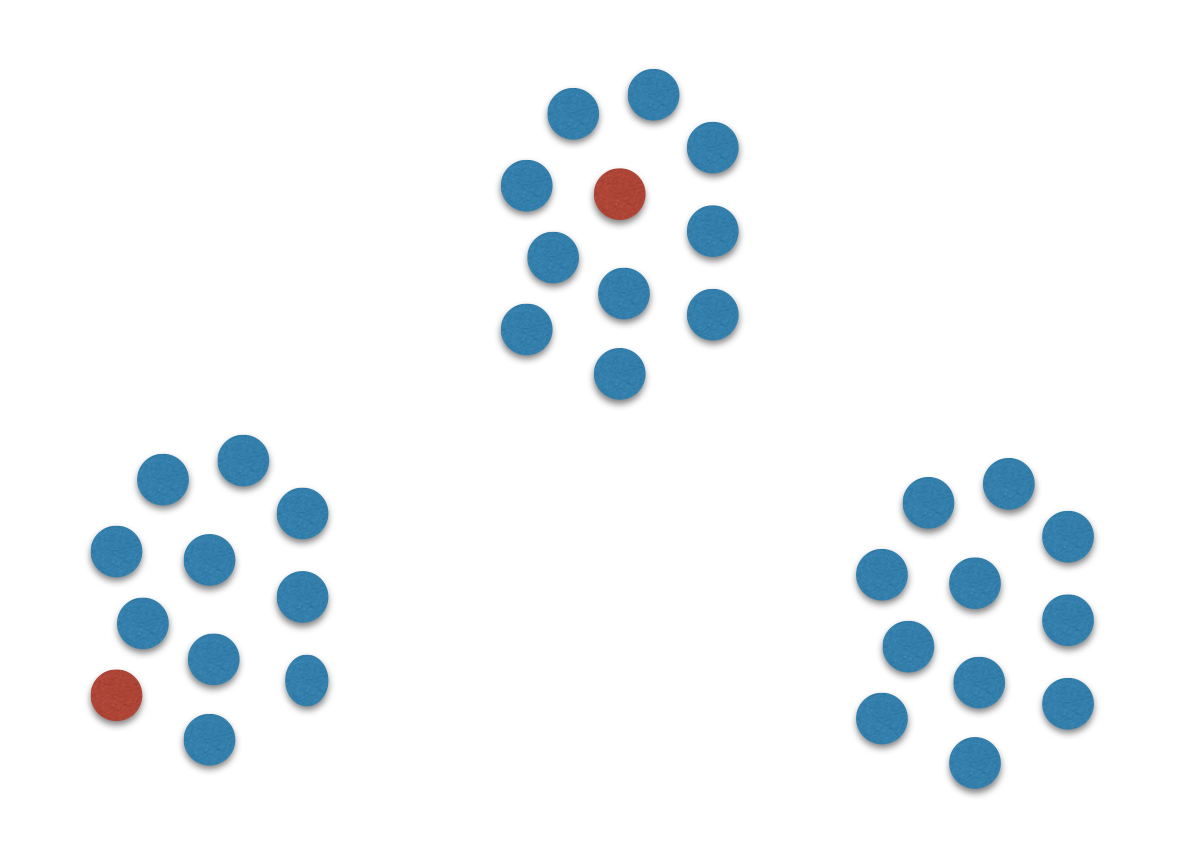
\includegraphics[ scale=0.25 ]{far.jpg}
			\caption{Finding point far from the chosen centroids}
			\label{fig:far_centroids}
		\end{subfigure}%
		\begin{subfigure}[H]{.5\textwidth}
			\centering
			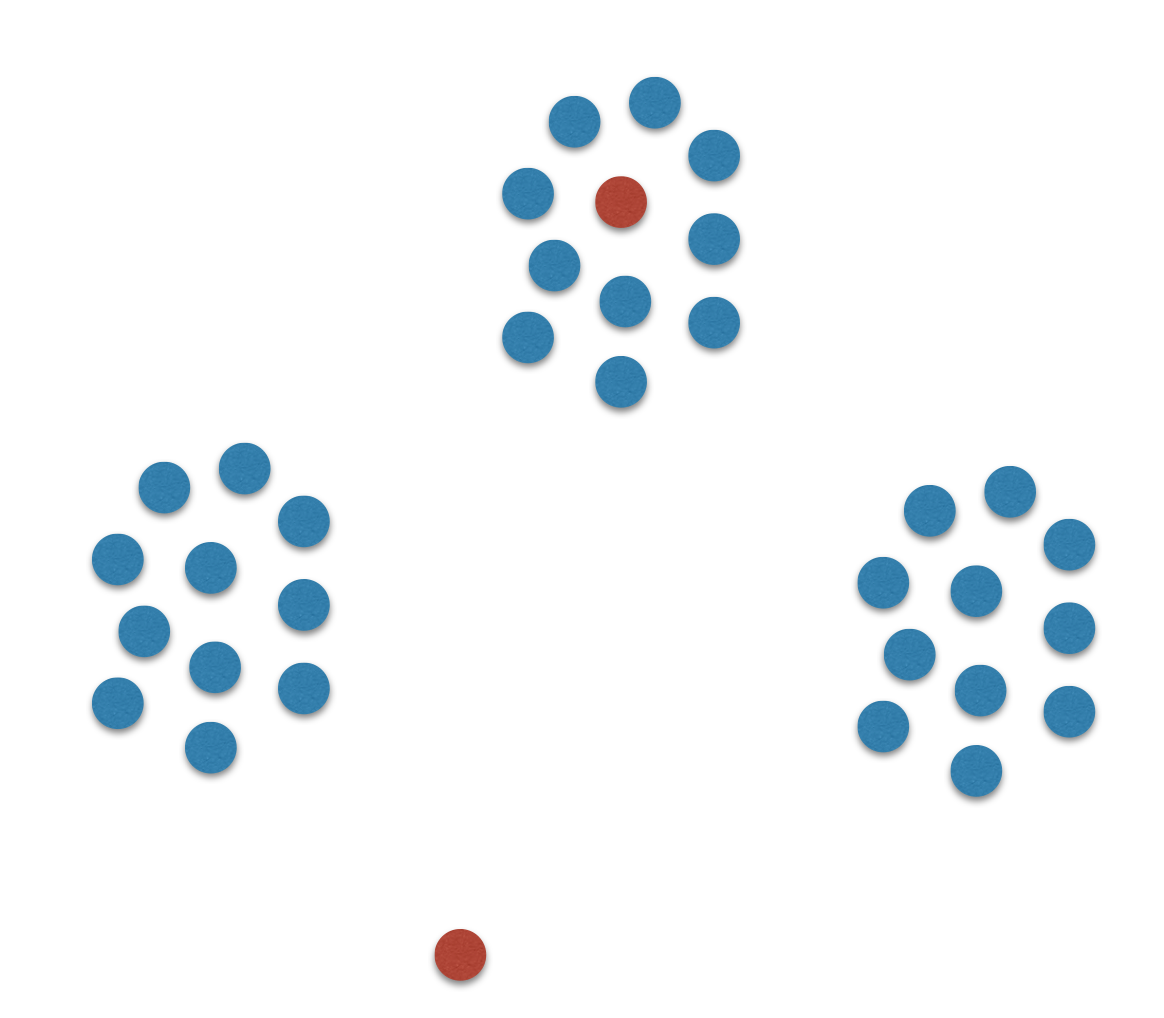
\includegraphics[ scale=0.2  ]{farthest.jpg}
			\caption{May choose the outlier point}
			\label{fig:ourlier_centroids}
		\end{subfigure}%
		\caption{How to choose the point?}
		\label{fig:centroids}
	\end{center}
\end{figure}
\item[Moving Average]

The definition of moving average is the following, \\
Given a window size $N_w$, and a sequence of real-valued number $S_i$ with size $N_s$, then the moving average sequence $M_i = \frac{\sum_{j=i}^{i+N_w} S_j}{N_w}$, where $i \in [0, N_s-N_w]$. \\

For example, if there exists a sequence 1,2,3,4,5,6 and assume the window size is 3, then the moving average sequence is 2,3,4,5. \\

Now the following is an example to show how to use moving average to stop the Mini-Batch KMeans. Assume the sequence of objective value of batch training set is 1,2,3,1,2,3. Thus, by the definition of moving average, we can get the following sequence 2,2,2,2. This sequence tells us the moving average is very stable, and we can stop at the second calculation of moving average. In other words, we can stop at the 4th calculation of objective value of batch training set, which means our Mini-Batch KMeans algorithm can stop at the 4th iteration. \\

However, there barely are so beautiful sequences. Therefore, that's why we use  $ | \text{previous moving average} - \text{current moving average} | \leq \varepsilon $ to define the stop criterion.

\item[Euclidean Distance]

Both KMeans or Mini-Batch KMeans need to calculate Euclidean distance. And this calculation will take the most part calculation time($> 80\%$). Thus, it's  important to speed up the calculation of Euclidean distance. \\

Recall the equation of Euclidean distance $ \norm{\textbf{X} - \textbf{Y}}_2^2 = \norm{\textbf{X}}_2^2 - 2\textbf{X} \cdot \textbf{Y} + \norm{\textbf{Y}}_2^2 $.
If we can precompute $\norm{\textbf{X}}_2^2$ and $\norm{\textbf{Y}}_2^2$, we can improve performance. \\ 

Therefore, we can precompute $\norm{\textbf{X}_i}_2^2$ , where $\textbf{X}_i \in$ data set,  in the beginning. 
And before assigning all points to the nearest centroid, we also can precompute $\norm{\textbf{C}_j}_2^2$, where $\textbf{C}_j \in$ cluster set. \\

However, by the experiment, we can observe no a great improvement happened on the calculation of Euclidean distance. Therefore, we need to speed up the calculation of inner product.

\item[Inner Product]

Recall the equation of inner product $\textbf{X} \cdot \textbf{Y} = \sum_{i=1}^{d} x_i y_i$. We may write the following code to calculate, \\
sum = 0.0; \\
for (i = 0;i $<$ d;i$++$) \{ \\
sum $+= x[\text{i}] * y[\text{i}]$; \\
\} \\

Thus, the calculation is $O(d)$, precisely speaking d multiplications and d-1 additions. To use the traditional method to assign a label to every point, it will cost $O(d \times M \times C)$, where $M$ is the number of data point, and $C$ is the number of cluster.

To improve this calculation, we need to use the property of CPU -- SIMD (Single Instruction Multiple Data). In x86 of Intel CPU, SSE(Streaming SIMD Extension) is an implementation of SIMD. SSE is a collection of 128 bits(16 bytes) CPU registers. These registers can do the same operation simultaneously. Recall the byte number of float type in C is 4 bytes. Thus, we can image if we have two vectors of four dimension with float type, and we want to do inner product. To use SSE, we can do the multiplications in one CPU cycle. And it also can do additions in registers without moving data to the address of "sum". The application of SSE is not only the calculation of inner product, there are other vector calculations in KMeans approach, like the calculation of center. Fortunately, scikit-learn includes of "fast\_dot" function to let us not write a assembly code to implement fast inner product.
\begin{verbatim}









\end{verbatim}

\item[Lazy Label Assignment]

If looking detail, we can observe that there may be duplicate calculations of Euclidean distance when assigning labels to elements of batch set. This is because assuming the element was already assigned to a some cluster with indexing K in the last iteration, and the element was chosen again in the current iteration. The original algorithm will re-assign the element to the cluster with indexing K. Actually, this "re-assign" action will cause degrading the speed of KMeans. Therefore, if an element was already assigned in the previous iterations, and that element was chosen in this iteration, we won't have to calculate the "REAL" distance in some conditions, i.e. assign labels lazily. \\

Recall that two properties of triangle inequality, \\
\begin{center}
	\begin{figure}[H]
		\centering
		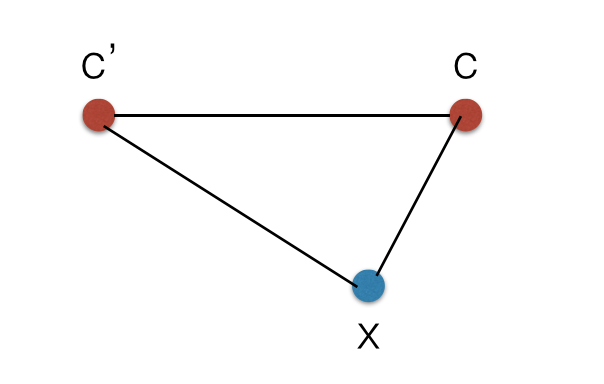
\includegraphics[scale=0.8]{triangle.jpg}
	\end{figure}
\end{center}
(1) if $d(c,c^{'}) \geq 2d(x,c)$ , then $d(x,c^{'}) \geq d(x,c)$ \\
(2) $d(x,c^{'}) \geq \max(0,d(x,c)-d(c,c^{'}))$ \\
\end{description}
Thus, we can generate an upper bound and lower bound of a distance. By using this concept, we can develop the following algorithm, \\

\begin{algorithm}[H]
	\caption{Lazy Label Assignment algorithm}
	\label{LazyLabel}
	\begin{algorithmic}[1]
		\Procedure {LazyLabelAssign} {$\textbf{X}_{d \times n}$, batch\_size}
		\State initialize lower bounds $L(\textbf{X}_{d \times n},c) \leftarrow d(\textbf{X}_{d \times n},c)$
		\State initialize upper bounds $U(\textbf{X}_{d \times n}) \leftarrow \min_c d(\textbf{X}_{d \times n},c)$
		\State initialize ownership $c(\textbf{X}_{d \times n}) \leftarrow \argmin_c d(\textbf{X}_{d \times n},c)$
		
		\For {t = 1 to T}
		\If { $ | \text{previous moving average} - \text{current moving average} | \leq \varepsilon $ }
		\State return $\bf{S}$
		\EndIf
		\State Choose a training set $\bf{X}_{Batch}$, and the size is batch\_size
		\For{ $x \in \bf{X}_{Batch} $ }
		\If { $ U(x) > L(x,c) $ and $ U(x) > \frac{1}{2} d(c(x),c) $, where $c \neq c(x)$ }
		\State calculate Euclidean distances of $d(x,c)$ and $d(x,c(x))$
		\If $d(x,c) < d(x,c(x))$
		\State $c(x) \leftarrow c$
		\EndIf
		\State $L(x,c) \leftarrow d(x,c)$
		\State $U(x) \leftarrow d(x,c(x))$
		\EndIf
		\EndFor
		\State calculate centroids $m(c)$ according to the batch set
		\For{ $x \in \bf{X}_{Batch} $ }
		\State $L(x,c) \leftarrow \max(0, L(x,c) - d(m(c), c))$, note: x has lower bound to each cluster
		\State $U(x) \leftarrow U(x) + d(c(x), m(c(x)))$
		\EndFor
		\EndFor 
		\State All points to be assigned label by calculating real Euclidean distance
		\State return final label
		\EndProcedure
	\end{algorithmic}
\end{algorithm}
%% ========================================
%% 		Subsection : VLAD
%% ========================================
%% 	=== description ===

\subsection {VLAD}
After we found the represent centroids of the whole database, which means the most-significent of patches of the dataset. The dimesion of centroids will depends on the patch size $l_{ps}^2$ and the number of centroids depends on the cluster number that we set from kmeans algorithm, represent as k here. In the following steps that we used a vector to represent each image by VLAD \cite{vlad}. In this approach, that we assign each local descriptor x to its nearest centroids first and one image have 200x200 patches (Here we represent as number m), which is described as algorithm \ref{NN} as $c_i = NN(x)$, that we apply the same methodology mentioned in kmeans algorithm before, which was already assign the nearest centroids label to each local descriptor x, and we only need to calcute the sum of all the grouped image descriptions by . 
\begin {equation}\label{nn_sum}
\bf{v_{i,j}} = \bf{\sum\limits_{\text{x such that label(x)} = c_i}}{x_j-c_{i,j}}
\end {equation}


%% 	=== algorithm ===

\begin{algorithm}[H]
	\caption{Nearest Neighbor}
	\label{NN}
	\begin{algorithmic}[1]
		\Procedure {NN} {$\bf{X}_{l_{ps}^2 \times m}, \bf{c}_{l_{ps}^2 \times k} , \bf{label}_m$}
		\State Intialize $\bf{group}_{k} \gets empty$
		\For{i = 1 to m}
		
		\State Assign difference to group[label[i]] 
		\State calculate the sum of each group by applying equation \eqref{nn_sum} for each $x_i$
		
		\EndFor
		\State return $\bf{group}$
		\EndProcedure
	\end{algorithmic}
\end{algorithm}

And the total flow of VLAD was described in algorithm \ref{VLAD}, which also implemeted the intra-normalization to suppress bursts. Because the repeated structure in the image will strongly affect the measure of similarity between two images since the repeated vector will contribute too much to decreased other important dimensions' contribution. This will especially effect a lot when we doing texture recognization because most of texture present duplicate pattern. This methodology was proposed from paper \cite{vlad_normalized}. The original normalization mentioned in paper \cite{vlad} was $L_2-normalized$ by $v:=v/\norm{v}_2$ 

\begin{algorithm}[H]
	\caption{VLAD}
	\label{VLAD}
	\begin{algorithmic}[1]
		\Procedure {VLAD} {$\bf{X}_{l_{ps}^2 \times m}, \bf{c}_{l_{ps}^2 \times k} , \bf{label}_m$}
		\State Intialize $\bf{result}_{k} \gets empty$
		\For{each $\bf{item}_{l_{ps}^2 \times k}$ in $NN(X,c,label)$}
		\For{each $\bf{block}_{l_{ps}^2}$ in item}
		\State intra-normalization for each block
		\EndFor
		\State Flatten as $\bf{VLAD}_{l_{ps}^2*k}$ for each image
		\State L2 normalization and append to result
		\EndFor
		\State return $\bf{result}$
		\EndProcedure
	\end{algorithmic}
\end{algorithm}





\subsection {Experiments Result}


There are six parameters in the program, i.e. window size, class size, subsample size, training ratio,  cluster number.
The following is the definitions of those parameters.
\\ \par 1. Window Size : the size of filter of extract local feature, also known as patch size. 
\\ \par 2. Class Size : There are 61 classes in our dataset.
\\ \par 3. Subsample Size : There are 92 images in each class.
\\ \par 4. Training Ratio : The ratio of size of training and testing 
\\ \par 5. Cluster Number : The size of bag of words.
\\ \par 6. Neighbor Number for Knn : The size of bag of words.


I sweeped cluster number in the sequence 4, 16, 32, 64, 128.
And for each cluster number, I sweep the neighbor number in the sequence 1 , 4 , 16, 32.
\\ \par
\begin{figure}[H]
	\begin{center}
		\begin{subfigure}{.5\textwidth}
			\centering
			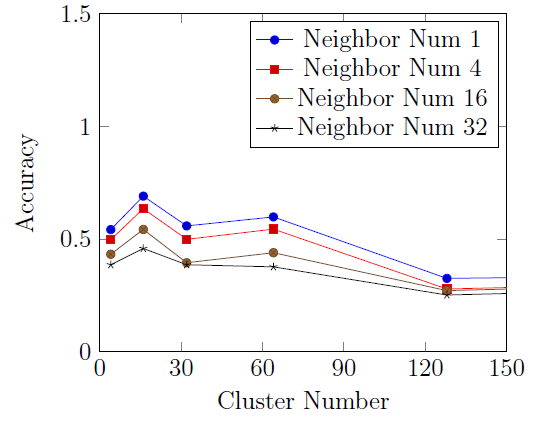
\includegraphics[ scale=0.5 ]{patch3.PNG}
			\caption{Accuracy when patch size =3}
			\label{fig:sub1}
		\end{subfigure}%
		\begin{subfigure}{.5\textwidth}
			\centering
			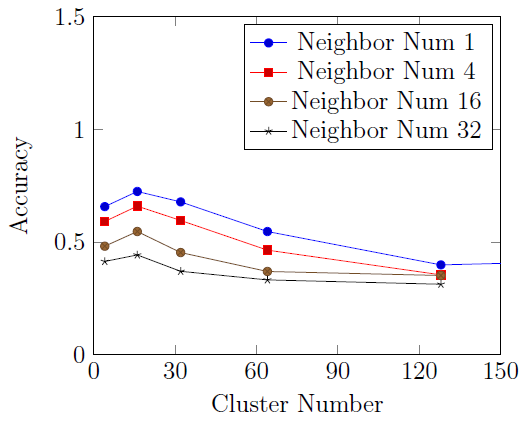
\includegraphics[ scale=0.5 ]{patch5.PNG}
			\caption{Accuracy when patch size =5}
			\label{fig:sub2}
		\end{subfigure}%
	\caption{Accuracy Between different patch sizes}
	\label{fig:patch}
	\end{center}
\end{figure}

\begin{figure}[H]
	\begin{center}
			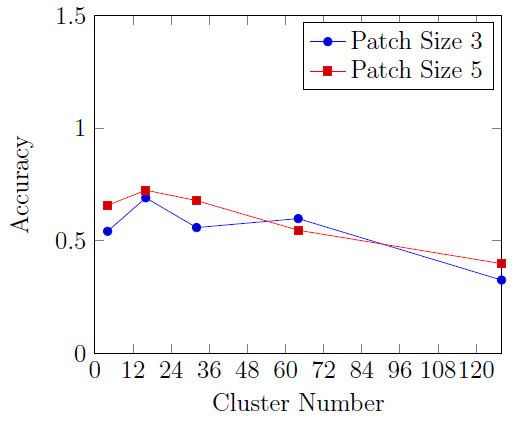
\includegraphics[ scale=0.5 ]{patchsize.PNG}	
	
	\caption{Compare Accuracy between Different Patch Size}
	\label{fig:comparePatch}
	\end{center}
\end{figure}

From the above figure, the optimal neighbor number of knn are both better when neighbor number is 1. And the cluster number is around number of 0 to 32 in this case. And we compared the performance between patch size equals to 3 and 5, we found there is better performance when patch size = 5. 
Therefore, we focused on the performance when patch size equals to 5, and used the neighbor number equals to 1 to take a deeper look at the accuracy change in this range.
\begin{figure}[H]
	\begin{center}
		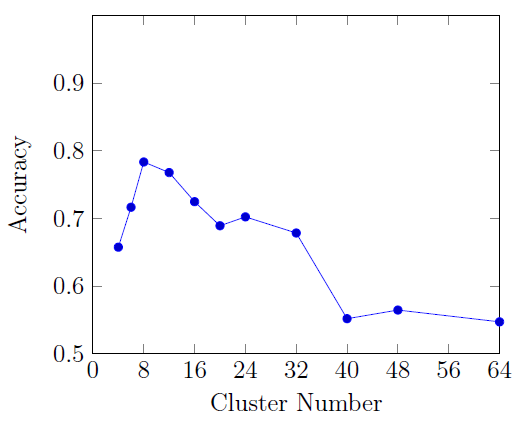
\includegraphics[ scale=0.5 ]{finetune.PNG}	
		
		\caption{ Accuracy when Patch Size = 5 and Neighbor number = 1}
		\label{fig:finetune}
	\end{center}
\end{figure}

According to \ref{fig:finetune}, in our experiment result for now, the best performance is about accurate rate = 80\%, when cluster number = 8, neighbor number = 1, patch size = 5.


\section{Baseline}
In our reference baseline \cite{baseline}, they used the CURet testure database, which we've obtained from the online \cite{dataset_mod}, including 61 classes of inage texture of $N=200^2$ pixels. And they used different classifiers to compares the error rates, with 46 training images over 92 images for each class.
The paper mainly focused on the performance of scattering PCA classifier, and which need to precompute the scattering coefficences and the scattering relies on three data structure: wavelet factories, layers, and filters. To represent effectively a signal, e.g. audio or image, scattering transform is a powerful tool. There is the software that we can directly reproduce their works \cite{baseline_software}. 
The tool provided below functions that we can step by step to implement, however, not every step there are clear instructions and the image demo example \cite{baseline_software} was based on a totally differet example, and we even don't know what's the settings for our baseline. To figure this, we first use linux command to find out all the scripts in the software by using "du -all $>$ fileslog", in this way, can track the function depedencies more efficient. The total flow included all the below steps was in the script \cite{github_flow}

\begin{description}
	\item[Loading data] 
	Loading images to process later, here we will use 61x92 images as input. But, there is not full instruction to tell you how to do the data preparation step by step. We had some clues from the image demo \cite{baseline_software} even that handled different dataset as ours. We figured out that there was already a function to store the each image path in the specified directory as a data structure also the sample class it belonged to. What we need to do was just simply modified the data process script fitted into our data description and path. \cite{github_data}
	\item[Wavelet operators] 
	From passing the settings in filt\_opt and scat\_opt to the factory, and the wavelet operators (Wop) can be obtained with 
	Wop = wavelet\_factory\_2d(size(x), filt\_opt, scat\_opt); If we wanted to replicate the exactly the same result as our baseline \cite{baseline}, we needed to find out what settings they used. Luckily, as we mentioned that we've listed all the scripts in this software, and we find out there were some scipts in the "paper" directory, which contains some original files to gereration the figures and tables for different paper, and from the paper \cite{baseline} setting for Figure 9, we could knew the setting in filt\_opt and scat\_opt to the factory. So that, we can generate the wavelet operators (Wop) with them.
	\item[Scattering transform] 
	Scattering transform depends on wavelet transform. The whole scattering tranformation system in this paper consists of two types of filter, one is low-pass filter, and the other is band-pass filter. The low-pass filter is based on Gaussian filter, and the band-pass filter is based on Morlet filter. For the low-pass filter, there are two parameters to control the amplitude and the bandwidth of filter response, i.e. J and Q. For the band-pass filter, there are three parameters to control, i.e. J, Q, and L. The definition of Gaussian filter is
	\begin{equation}
		G(\alpha, u, v) = \alpha^2\phi(\alpha u, \alpha v)
	\end{equation}
	where $\alpha = 2^{-j/Q}, j \in [0, J-1], \phi $ is two-dimension Gaussian function.
	The definition of Morlet filter is
	\begin{equation}
		M(\alpha, \theta, u, v) = \alpha^2\psi(e^{j\theta} \alpha u, e^{j\theta}\alpha v)
	\end{equation}
	where $\alpha = 2^{-j/Q}, j \in [0, J-1], \theta = l/L \times \pi, l \in [0, L-1], \psi $ is two-dimension mother Morlet function.
	For every layer of scattering transform, there are two operations, one is signal filtered by Morlet filter bank, and then that signal filtered by Gaussian filter bank. The formal definition of scattering transform is the following:
	\begin{equation}
		S_m(u,v) = U_{m-1}(u,v) \star G(\alpha, u, v)
	\end{equation}
	
	\begin{equation}
		S_0(u,v) = Image(u,v) \star G(\alpha, u, v)
	\end{equation}
	
	where 
	
	\begin{equation}
		U_m(u,v) = U_{m-1}(u,v) \star M(\alpha, \theta, u, v)
	\end{equation}
	
	\begin{equation}
		U_0(u,v) = Image(u,v) \star M(\alpha, \theta, u, v)
	\end{equation}
	
	and m is the scattering network layer index.
	
	If we choose larger m, we can get higher frequency features. But, the most energy of images is near lower frequency, so the default value of m is 2. For each m-th layer, we have $J \times L$ node according to different $j \in [0, J-1]$ and $l \in [0, L-1]$.
	Thus, the time complexity is $O((N \times J \times L)^m)$, where N is the total pixel number of an image.
	After calculating scattering transformation, we have concatenated all parameter to produce scattering vector, i.e. the feature vector of an image.
	\begin{equation}
		S_{coef} = (S_0, S_1, ..., S_m) 
	\end{equation}
	where $S_m$ is also a vector $ (S_m^{0}, S_m^{1}, ..., S_m^{JL}) $, and for each $S_m^{i}$ is the calculation of norm-1 of the convolution result, i.e. 
	$S_m^{i} = | U_{m-1}^{i}(u,v) \star G(\alpha_i, u, v) |_1$. Thus, we can think scattering vector as a collection of energy distribution according to different J and L. Thus, we can see the color variation of the scattering coefficients display in the paper. The darker region means the most energy centralize in this region given specific parameters J and L. Therefore, this recognition method is mainly based on that two similar textures would have the similar energy distribution. 
	By calling the scat function to computethe scattering of x using Wop defined in the last step. Basically, the scattering coefficients are computed with for each sale variable J and each rotation angle variable $\theta$, and also with default $m_{max}$ value in scat\_opt.M = 2;
	\item[Classification] 
	Performs an affine PCA classifier using the feature computed from previous steps and reformed as 3D matrix by separating 50/50 of the training and testing data. The first thing we needed to do is data preparation by feeding the each image stored in src structure and the feature function created before, used these as input feature to train the half of data to generate the model. After that, used this model to test the rest of half of data, can finally report the error rate between them. In our case, we got the error rate about 0.041 when $M_{max} = 2$, which is 4 \% and larger than the original 0.2\%, also we got the error rate 98.36 \% when $M_{max} = 1$. We suspected that the larger error rate came from our fewer data than original. We tried to use $M_{max} = 3$ to achieve better error rate, however, we encountered obstacle to get the result becasue it consumed really long time and kept disconnecting by networking and server probelm. We figured out the running time will be $O((200 \times 7 \times 8)^3) = 1.404928e+12$ for one picture, and there are still 854 pictures after trimmed. 
\end{description}

	\begin{table}[htbp]
		\caption{Percnetage of erros on CURet for different training sizes \\
		And different method	}
		\label{baseline_evaluation}
		\begin{center}\footnotesize
			\renewcommand{\arraystretch}{1.3}
			\begin{tabular}{|c|c|c|c|c|c|}\hline
				\makecell{ VLAD \\ \bf KNN} &
				\makecell{ X \\ \bf PCA} & 
			    \makecell{ $Scat. M_{max} = 1$ \\ \bf PCA} & 
			    \makecell{\bf $Scat. M_{max} = 2$ \\  \bf PCA} & 
			    \makecell{\bf $Scat. M_{max} = 2$ \\  \bf PCA by training size only 7}\\ \hline\hline
				23\% & 17\% & 0.05\% & 0.02\% &  4\% \\\hline
			
			\end{tabular}
		\end{center}
	\end{table}

In spite of researching in the software usage itself, We spent a lot of time in setting all the simulation enviorment. At first, we've already have HPC account, so we directly used the matlab on the machine, however we had problem to show the picture in our local, so we searched for the ForwardX setting to make the matlab can execute as GUI interface in our local computer. After that, when we started to run our experiement, it still costed a long time to report the result even we already used HPC machine. So that we decided to trim the data left only the first 14 pictures for each sample, in this way, we can at least have a rough result to check our flow is ok or not. And by these subdata set ran in HPC cost about at least half of hour to get the result depends on different $Scat. M_{max}$ settings, larger will cost longer time to compute. But we encountered server problem that we should run long jobs with PBS script to run on compute nodes instead of login node when we tried to do $M_{max} = 3$ experiment. So we also set up the script for our future project usage.
In additions, for collaboration efficency, we uploaded all our scripts on the github \cite{github}, this also helped us when we changed from different machines and accounts. 

%\begin{verbatim}





%\end{verbatim}


\section{Conclusion} 
All our codes and experiments script could be found in the github link \cite{github_final}. And in each folder contains the temporary results of each steps in our pipeline. And compare the performance with baseline, we have lower accurate rate but with optimized run-time by implementing the methodologies mentioned in optimization of kmeans section. By this way, we not only improve the run time of kmeans cacluation but also take advantage of lazy label assignment when kmeans to speed up the process of getting VLAD. From the comparision run-time table \ref{time} based on  patch size = 3, class number = 10 , 2 images for each class , we can see the timing from both achieve reducing 80\% of runtime in mini-batch kmeans and get VLAD. And also only 1/3 of time compared with our baseline when extracted the features.

\begin{table}[htbp]
	\caption{Time-consuming (Seconds)}
	\label{time}
	\begin{center}\footnotesize
		\renewcommand{\arraystretch}{1.3}
		\begin{tabular}{|c||c|c|c|c|}\hline
			{\bf \makecell{ Process \\ \bf Tools} }  & Extract Patch & Kmeans & Get Vlad & Knn\\ \hline 
			Ours  & 6.45
			& $89 \rightarrow13$ & $70 \rightarrow13$ & NaN \\ \hline
			Scikit Learn  & NaN &  12 & NaN & 0.1\\  \hline
			
			Baseline  & \multicolumn{3}{c|}{81.18} & NaN\\  \hline
			
		\end{tabular}
	\end{center}
\end{table} 

\begin{verbatim}

















\end{verbatim}

\begin{thebibliography}{1}

\bibitem{baseline} {\sc J.Bruna and S. Mallat}, {\em Invariant Scattering Convolution Network}, CMAP, Ecole Polytechnique, Palaiseau, France


\bibitem{dataref} {\sc M.Varma, A. Zisserman}, {\em A Statistical Approach To Material Classification Using Image Patch Exemplars}, IEEE Trans. on
PAMI, 31(11):2032–2047, November 2009.

\bibitem{dataref_mod} {\sc M. Varma and A. Zisserman}, {\em A statistical approach to texture classification from single images}, International Journal of Computer Vision, vol. 62, no. 1-2, pp. 61–81,
2005.

\bibitem{dataset} {\sc K.J. Dana, B. Van-Ginneken, S.K. Nayar, J.J. Koenderink}, {\em Reflectance and Texture of Real World Surfaces,}, ACM Transactions on Graphics (TOG),
Vol.18, No.1, pp.1-34, Jan, 1999.

\bibitem{dataset_link} {\em http://www.cs.columbia.edu/CAVE/software/curet/}

\bibitem{dataset_mod}{\em http://www.robots.ox.ac.uk/~vgg/research/texclass/data/curetgrey.zip}

\bibitem{l1l0} {\sc C Ramirez, V Kreinovich, M Argaez}, {\em  Why l1 Is a Good Approximation to l0: A Geometric Explanation}, Journal of Uncertain Systems 7 (3), 203-207, 2013. 3, 2013.

\bibitem{baseline_software}{\em http://www.di.ens.fr/data/software/scatnet/quickstart-image/}

\bibitem{book} {\sc J. Mairal, F. Bach, and J. Ponce}, {\em  Sparse Modeling for Image and Vision Processing}, Foundation and Trends in Computer Graphics and Vision, 2014.

\bibitem{github} {\em https://github.com/chialingwang/ML\_textureRecognize}
\bibitem{github_data} {\em https://github.com/chialingwang/ML\_textureRecognize/blob/master/papers/ISCV/curet\_src.m}

\bibitem{github_flow} {\em https://github.com/chialingwang/ML\_textureRecognize/blob/master/papers/ISCV/classification.m}

\bibitem{triangle} {\sc C. Elkan } , {\em Using the Triangle Inequality to Accelerate k-Means} , Department of Computer Science and Engineering

\bibitem{vlad_normalized} {\sc R. Arandjelovic. A. Zisserman } , {\em All about VLAD} , Department of Engineering Science, University of Oxford

\bibitem{vlad} {\sc H. Jegou, M. Douze, C. Schimid, and P. Perez } , {\em Aggregating Local. Descriptors into a Compact Image Representation} , CVPR, 2010

\bibitem{github_final} {\em https://github.com/chialingwang/ML\_Project}

\end{thebibliography}


\end{document}
%% end of file `projectProposal.tex'
